\documentclass[12pt]{article}

%%%%%%%%%%%%%%%%%%%%%%% Don't change anything in here. This space is called the preamble, it is where you tell the computer to load the proper LaTeX packages to perform the math and formatting desired. 
\usepackage{url}
\usepackage{multicol}
\usepackage{amsmath}
\usepackage{esint}
\usepackage{physics} 
\usepackage{siunitx}
\usepackage{bigints}
\usepackage{amsfonts}
\usepackage{textcomp}
\usepackage{xcolor}
\usepackage{tikz}
\usepackage{verbatim}
\usetikzlibrary{calc}
\usetikzlibrary{decorations.pathmorphing}
\usepackage{amsmath,amssymb}
\usepackage{siunitx} 
\usepackage{subcaption} 
\usepackage{blindtext} 
\usepackage{enumerate} 
\usepackage{pgfplots}
\usepackage{graphicx}
\usepackage{dsfont}
\usepackage{float}
\bibliographystyle{iopart-num}
\usepackage{cite}
\usepackage{wrapfig} %preámbulo
\usepackage{enumitem}
\usepackage{pgfplotstable}
\usepackage[compact]{titlesec}  
\usepackage[document]{ragged2e}
\usepackage{tikz,pgfplots}
\usepackage[spanish]{babel}
\usepackage[utf8]{inputenc}
\usepackage{hyperref}
\usepackage{amsmath, amsthm, amssymb}  %I added this so that you can use the align tool for equations!
\usepackage{colortbl}
\usepackage{mathtools}
\usepackage{sectsty}
\usepackage{esint}
\usepackage[makeroom]{cancel}
\usepackage{pgfplots}
\usepackage{graphicx}
\usepackage{dsfont}
\usepackage{float}
\usepackage{pdfpages}
\bibliographystyle{iopart-num}
\usepackage{cite}
\usepackage{wrapfig} %preámbulo
\usepackage{enumitem}
\usepackage{pgfplotstable}
\usepackage[compact]{titlesec}  
\usepackage[document]{ragged2e}
\usepackage{tikz,pgfplots}
\usepackage[spanish]{babel}
\usepackage[utf8]{inputenc}
\usepackage{hyperref}
\newtheorem{thm}{Teorema}[subsection]
\newtheorem{teo}[thm]{Teorema}
\newtheorem{obss}{Obs}[subsection]
\newtheorem{defff}{Def}[subsection]
\newtheorem{conjeture}{Conj}[subsection]
\newtheorem{defn}[defff]{Definición}
\newtheorem{lem}{Lemma}[thm]
\newtheorem{cor}{Corollary}[thm]
\newtheorem{prop}{Proposition}[thm]
\newtheorem{rem}{Remark}[thm]
\newtheorem{ill}{Illustration}[thm]
\newtheorem{conj}[conjeture]{Conjetura}
\newtheorem{obs}[obss]{Observación}
\usepackage{amsmath, amsthm, amssymb}  %I added this so that you can use the align tool for equations!
\usepackage{geometry}
 \geometry{
 a4paper,
 total={170mm,257mm},
 left=20mm,
 top=20mm,
 }
\pgfplotsset{compat=1.14}
\graphicspath{ {images/} }
%%%%%%%%%%%%%%%%%%%%%%%%% Again, Don't change anything Above %%%%%%%%%%%%%%%%%%%%
\newcommand{\eq}[1]{\[#1\]}
\newcommand{\s}[1]{\section{#1}}
\newcommand{\en}[1]{\[\boxed{#1}\]}
\newcommand{\coss}[1]{\cos{\qty(#1)}}
\newcommand{\mc}[1]{\mathcal{#1}}
\newcommand{\md}[1]{\mathds{#1}}
\newcommand{\sinn}[1]{\sin{\qty(#1)}}
\newcommand{\lnn}[1]{\ln{\qty(#1)}}
\newcommand{\intt}[2]{\int\limits_{#1}^{#2}}
\newcommand{\ointt}[2]{\oint\limits_{#1}^{#2}}
\newcommand{\sumn}[1]{\sum_{#1 =1}^{n}}
\newcommand{\summ}[2]{\sum_{#1 =1}^{#2}}
\newcommand{\pp}[2]{\vec{#1}\cdot\vec{#2}}
\newcommand{\pc}[2]{\vec{#1}\, \cross\, \vec{#2}}
\newcommand{\eva}[3]{\eval{#1}_{#2}^{#3}}
\renewcommand{\ss}[1]{\subsection{#1}}
\newcommand{\sss}[1]{\subsubsection{#1}}
\newcommand{\xn}[1]{{#1}_{1},{#1}_{2},\cdots,{#1}_{n}}
\newcommand{\so}{\[\textrm{\textbf{Solución}} \]}
\newcommand{\ej}{\[\textrm{\textbf{Ejemplo}} \]}
\newcommand{\vl}{\,\,\, \vline \,\,\,}
\newcommand{\ob}{ \textit{\textbf{Observación:}} \\}
\newcommand{\pua}{$\bullet \, $}
\newcommand{\eqreff}[1]{Ecuación [\ref{#1}]}
\newcommand{\fgref}[1]{Figura [\ref{#1}]}
%%%%%%%%%%%%%%%%%%%%%%%%%%%%%%5
% Creación de colores
\definecolor{rojo}{RGB}{255, 0, 0}
\definecolor{negro}{RGB}{0, 0, 0}
\definecolor{burdeo}{RGB}{231, 76, 60}
\definecolor{fucsia}{RGB}{255, 0, 171}
\definecolor{morado}{RGB}{142, 69, 212}
\definecolor{verde}{RGB}{26, 139, 73}
\definecolor{violeta}{RGB}{155, 89, 182}
\definecolor{celeste}{RGB}{0, 176, 255}
\definecolor{azul}{RGB}{18, 3, 119}
\definecolor{azul_fosfo}{RGB}{10, 0, 255}

%%%%%%%%%%%%%%
%Colores%
\newcommand{\rojo}[1]{{\color{rojo}#1}}
\newcommand{\negro}[1]{{\color{negro}#1}}
\newcommand{\azul}[1]{{\color{azul}#1}}
\newcommand{\verde}[1]{{\color{verde}#1}}
\newcommand{\burdeo}[1]{{\color{burdeo}#1}}
\newcommand{\rosa}[1]{{\color{fucsia}#1}}
\newcommand{\morado}[1]{{\color{morado}#1}}
\newcommand{\violeta}[1]{{\color{violeta}#1}}
\newcommand{\celeste}[1]{{\color{celeste}#1}}
\newcommand{\azulf}[1]{{\color{azul_fosfo}#1}}
%%%%%%%%%%%%%%%%%%%%%%%%%%%%%%%%%%%%%%%
%%%%%%%%%%%%%%%%%%%%%%%%%%%%%%%%%%%%%%%%%

%%Figuras
\begin{comment} %Figura
\begin{figure}[h!]
    \centering
    \includegraphics[width=0.5\textwidth]{}
    \caption{}
    \label{}
\end{figure}
\end{comment}
%Importar PDF
\begin{comment}
 \includepdf[pages=(pagina inicial)-(pagina final)]{direccion de archivo}
\end{comment}
%%Comando para tachar con colores y señalar que se reemplazó
\begin{comment}
 Cancelar con colores ; \Cancel[blue]{2}+\Cancel[red]{1}-
 \Cancel[blue]{2}-\Cancel[red]{1}\\
 
 Cancelar normal; \Cancel{x}\\
 
 Cancelar con una cruz; \xCancel{}\\
 
 Cancelar e indicar con qué valor se reemplazó ; \cancelto{Se vuelve esto}{Reemplaza esto}\\
 Separar la hoja con una raya negra: \hline 
 Separar la hoja con puntos negros: \dotfill
 
\end{comment}
%%%%%%%%%%%%%%%%%%%%%%%%5

% Derivadas
\begin{comment}
 n-esima Derivada Normal (si quieres la normal borra el [n]); \dv[n]{f}{x} \\
 n-esima derivada parcial (si quieres la normal borra el [n]) : \pdv[n]{f}{x}\\
 derivada mixta: \pdv{f}{x}{y}  \\
\end{comment}
%%%%%%%%%%%%%%

%Integral: 
\begin{comment}
 Integral de linea con limites inferior y superior: \oint \oiint \limits_{}^{}
\end{comment}
%%%%%%%%%%%%%




\begin{document}

%%ESTO ES EL ENCABEZADO
\begin{flushleft}
    \begin{figure}[t]
    \raggedright

\includegraphics[scale=0.2]{Logo_UTFSM.png}
    \label{fig:imagen}
\end{figure}
\end{flushleft}

\begin{flushright}
\vspace{-4cm}
\hspace{8cm}
\textbf{Universidad Técnica Federico Santa María\\
\hspace{9cm}Departamento de \textbf{Física}\\
\hspace{9cm}FIS210\\
\hspace{9cm}2°. Semestre 2021}
\end{flushright}

\begin{center}
    \large
    %TITULO DEL PAPER%
    \textbf{FIS210: Clase 21 }\\
    \large
    \author[Bastián Castorene$^1$\\
    \today\\
    {$^1$\small{\textit{Estudiante de Licenciatura en Física, Departamento de Física, UTFSM}}}\\
\end{center}
\s{Transformaciones Canonicas}
En el lagragiano uno puede cambiar las coordenadas y las ecuaciones resultantes tendrán la misma forma.\\
En el formalismo Hamiltoniano pasa lo mismo, se pueden cambiar las coord. generalizadas pero igual se deben cambiar los momentos generalizados.\\
\en{\textit{Por ahora 1 grado de libertad}}
$$\mathcal{H}(q,p) \implies \dot{q}=\pdv{\mathcal{H}}{p}\,\,\vline \,\, \dot{p}= \pdv{\mathcal{H}}{q} $$ 
Que posibilidades hay de cambiar las coordenadas
\eq{q,p \rightarrow Q,P}

Tales que 

$$\mathcal{H}(Q,P) \implies \dot{Q}=\pdv{\mathcal{H}}{P}\,\,\vline \,\, \dot{P}= \pdv{\mathcal{H}}{Q} $$ 
Forma canonicas de las ecuaciones de hamilton.\\
No cualquier cambio funciona para esto, pero si lo logra se llaman Transformaciones canonicas.\\
\begin{align}
P= P(q,p) \implies \dot{P} = \pdv{P}{q} \dot{q}+ \pdv{P}{p}\dot{p}\\
\dot{P}= \pdv{\mathcal{H}}{Q}	= - \qty(\pdv{\mathcal{H}}{q} \pdv{q}{Q}+ \pdv{\mathcal{H}}{p}\pdv{p}{Q})\\
\dot{P}= \dot{p}\pdv{q}{Q} - \dot{q} \pdv{p}{Q}\\
\dot{Q}+ \pdv{\mathcal{H}}{P}= \qty(\pdv{\mathcal{H}}{q} \pdv{q}{P}+ \pdv{\mathcal{H}}{p}\pdv{p}{P})\\
\dot{Q}= - \dot{p}\pdv{q}{P}+ \dot{q}\pdv{p}{P}
\end{align}
Si combinados todos los terminos semejantes obtendremos:\\
\begin{align}
\dot{q} \qty(\pdv{P}{q}+ \pdv{p}{Q})+\dot{p}\qty(\pdv{P}{p}- \pdv{q}{Q})=0\\
\dot{q} \qty(\pdv{Q}{q}- \pdv{p}{P})+\dot{p}\qty(\pdv{Q}{p}+ \pdv{q}{P})=0
\end{align}
Tenemos un sistema lineal de ecuaciones con solucion no trivial cuando el determinante de la matriz es cero.
\begin{align}
&\begin{vmatrix}
\qty(\pdv{P}{q}+ \pdv{p}{Q})&	\qty(\pdv{P}{p}- \pdv{q}{Q})\\
\qty(\pdv{Q}{q}- \pdv{p}{P})& \qty(\pdv{Q}{p}+ \pdv{q}{P})
\end{vmatrix}=0\\
&\qty(\pdv{P}{q}+ \pdv{p}{Q})\cdot \qty(\pdv{Q}{p}+ \pdv{q}{P})- \qty(\pdv{Q}{q}- \pdv{p}{P})\cdot \qty(\pdv{P}{p}- \pdv{q}{Q})= 0\\
&\qty(\pdv{P}{q} \pdv{Q}{p}-\pdv{P}{p} \pdv{Q}{q})+ \qty(\pdv{p}{Q} \pdv{q}{P}-\pdv{q}{Q} \pdv{p}{P})+\underbrace{\qty(\pdv{P}{q} \pdv{q}{P}+ \pdv{P}{p} \pdv{p}{P})}_{1} +\underbrace{\qty(\pdv{Q}{p} \pdv{p}{Q}+ \pdv{Q}{q} \pdv{q}{Q})}_{1}\\
& \qty(\pdv{P}{q} \pdv{Q}{p}-\pdv{P}{p} \pdv{Q}{q})+ \qty(\pdv{p}{Q} \pdv{q}{P}-\pdv{q}{Q} \pdv{p}{P})+2 \label{po1}
\end{align}
Es hora de ingresar la notacion del Corchete de Poisson.\\
f(q,p) y g(q,p).
\begin{align}
[f,g]= \pdv{f}{q} \pdv{g}{p}-\pdv{f}{p} \pdv{g}{q}
\end{align}
Si introducimos esta notaciónen \eqreff{po1} tenemos:
\begin{align}
[P,Q]_{q,p}+[p,q]_{Q,P}+2=0	\label{po2}
\end{align}
$$[P,Q]_{p,q}\, \textit{Es el determinante del Jacobiano de la transformacion del cambio de variable }$$
$$p,q \rightarrow P,Q $$

$$[p,q]_{p,q}\, \textit{Es el determinante del Jacobiano de la transformacion \textbf{Inversa} del cambio de variable }$$
$$[p,q]_{Q,P} = \qty(\,[P,Q]_{q,p}\, )^{-1} $$
Si ahora introducimos esta propiedad del inverso del Jacobiano en la \eqreff{po2} tenemos:
\begin{align}
[P,Q]_{q,p}+ \qty([P,Q]_{q,p})^{-1} + 2 =0\bigg/\cdot [P,Q]_{q,p}\\
\qty([P,Q]_{q,p})^2+ \cancelto{1}{[P,Q]_{q,p}\qty([P,Q]_{q,p})^{-1}} + 2 [P,Q]_{q,p} =0\\
\qty([P,Q]_{q,p})^2+ 2 [P,Q]_{q,p} +1 =0\\
\qty([P,Q]_{q,p}+1)^2=0
\end{align}
\en{[P,Q]_{q,p}=-1}
O equivalentemente, porque el corchete de Poisson es anti conmutativo:
\en{[Q,P]_{q,p}=1}
O equivalentemente

\en{[q,p]_{Q,P}=1}
$\therefore$ una transformacion es canonica si se cumple cualquiera de las 3 propiedades anteriores. 
\newpage

\ej
$$q,p \rightarrow \theta,J \bigg/ \frac{p^2}{2m}= J \omega \cos^2{(\theta)} \bigg/ \frac{k}{2}q^2= J \omega \sin^2{(\theta)}$$
$$\omega^2+\frac{k}{m} $$
Si la transformación  fuera canonica nos simplificaria todo el Hamiltoniano.Lo es?\\
Procedemos a despejar las variables q y p.
\begin{align}
q= \sqrt{\frac{2J \omega}{k}} \sinn{\theta}\,\, \vline \,\, p=\sqrt{2m\omega J} \coss{\theta}	\label{op4}
\end{align}
Ahora calculamos el corchete de Poisson de las nuevas coordenadas.\\
\begin{align}
[p,q]_{\theta,J} &= \pdv{p}{\theta} \pdv{q}{J}-\pdv{p}{J} \pdv{q}{\theta}\\
	&=-\sqrt{2m\omega J}\sinn{\theta} \frac{1}{2} \sqrt{\frac{2\omega}{J k}} \sinn{\theta} - \frac{1}{2} \sqrt{\frac{2\omega}{J}} \coss{\theta} \sqrt{\frac{2J\omega J}{k}}\coss{\theta}\\
	&=-1
\end{align}
$\therefore$ Se verificó que esta transformación es canonica.
\begin{align}
\mathcal{H}=J \omega \,\, \vline \,\, \dot{\theta}=\pdv{\mathcal{H}}{J}=\omega	
\end{align}
La ecuacion quedo extremadamente sencilla, aunque claro, nos sacamos esta transformacion de la manga.
$$\theta = \omega t + \phi_n$$


$$\dot{J} = - \pdv{\mathcal{H}}{\theta} \implies J= \textit{Const}$$

Si introducimos este resultado en la \eqreff{op4} tenemos:
\begin{align}
q= \sqrt{\frac{2J \omega}{k}} \sinn{\theta}= \sqrt{\frac{2E}{k}} \sinn{\omega t + \phi_n}\\
p= \sqrt{2mE} \coss{\omega t + \phi_n}
\end{align}	
Encontramos las soluciones del oscilador armonico. con un metodo novedoso. \\
Si visualizamos el espacio de fases en terminos de las nuevas coordenadas tenemos a diferencia de las elipses de las coordenadas originales:

\begin{figure}[h!]
    \centering
    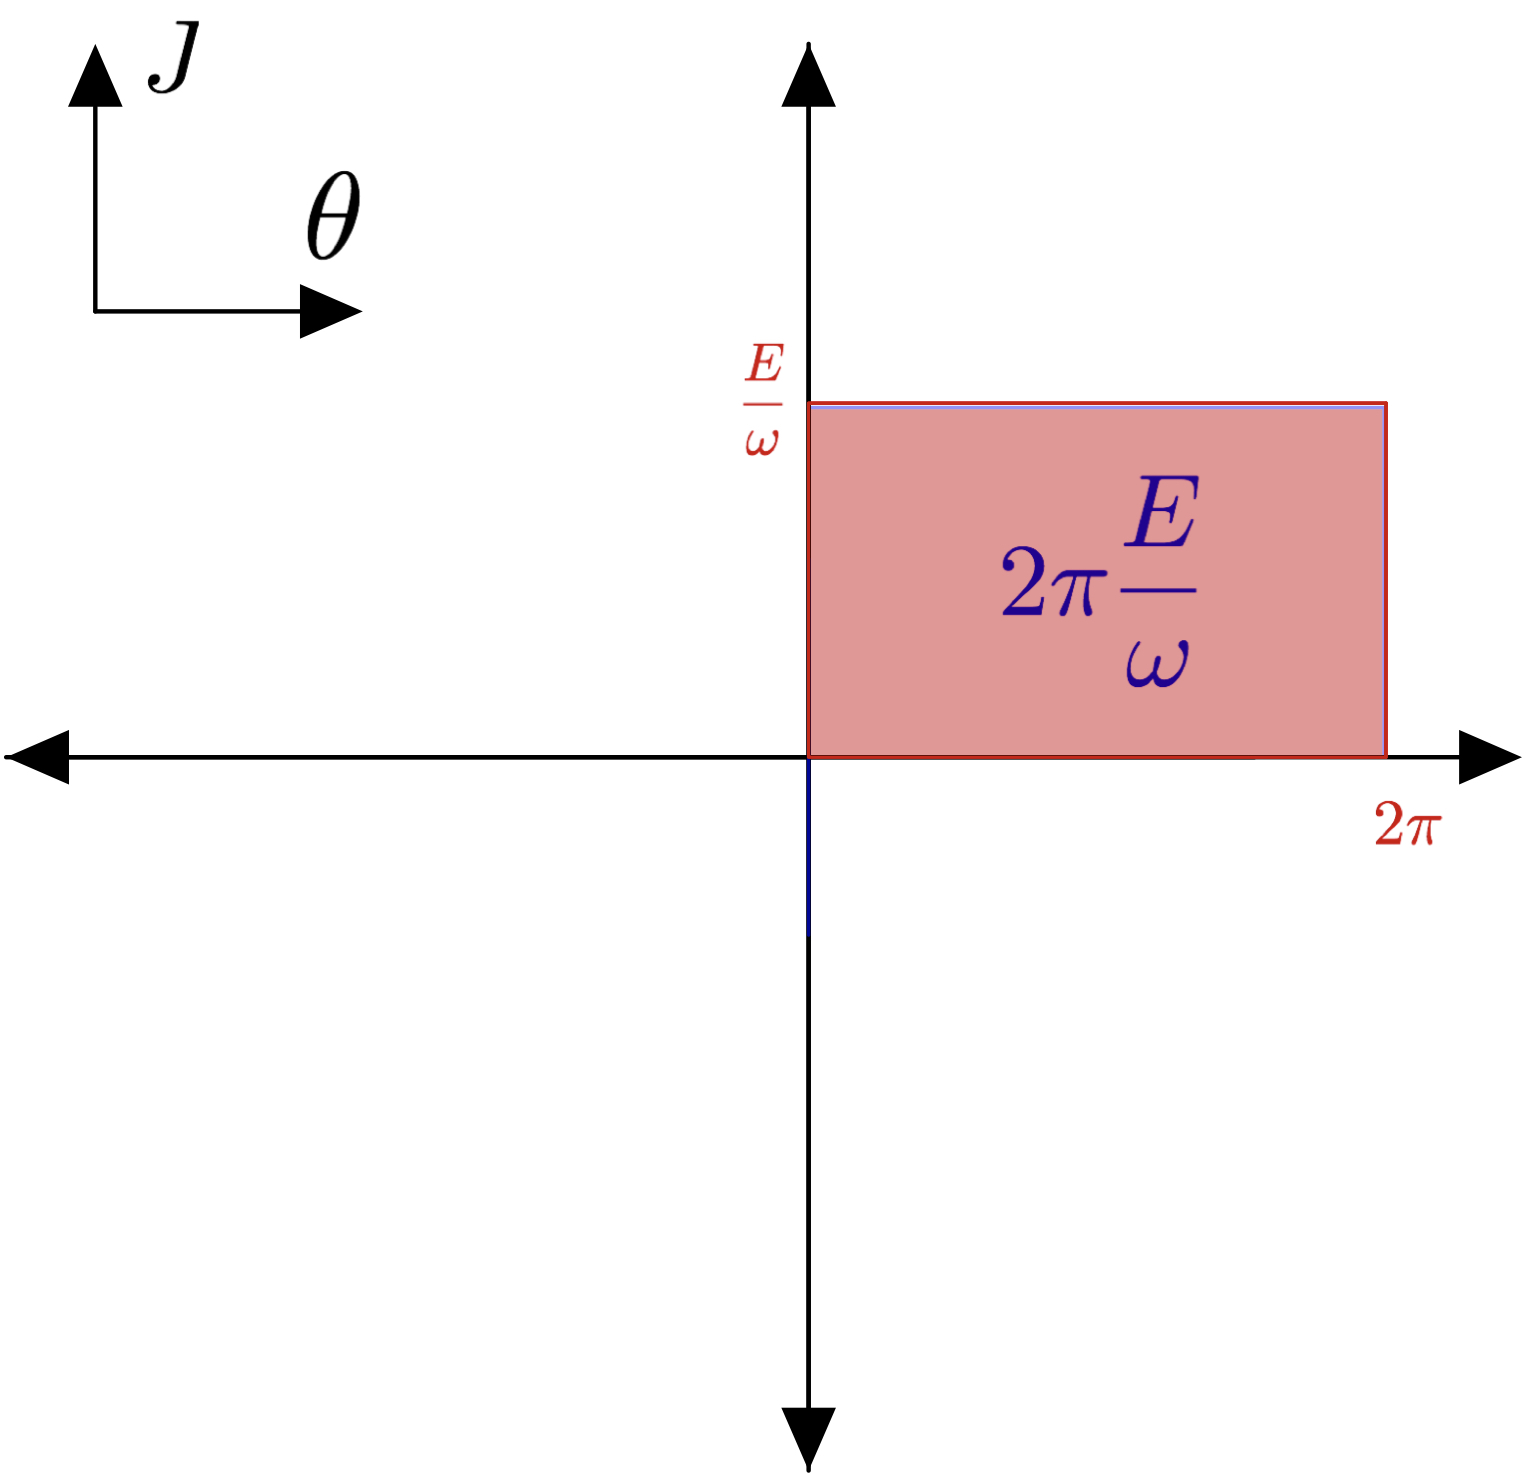
\includegraphics[width=0.3\textwidth]{edf_jt.png}
    \caption{Espacio de fases q,p nuevas}
    \label{edf_jt}
\end{figure}

Se puede observar es que en la nuevas variables, la elipse se aplanó y el área es igual. \\
si pudieramos encontrar coord y momentos que nos aplanen los espacios de fases sería maravilloso.\\
\pagebreak
\s{Corchetes de Poisson}

f(q,p) y g(q,p).
\begin{align}
[f,g]= \pdv{f}{q} \pdv{g}{p}-\pdv{f}{p} \pdv{g}{q}
\end{align}
Se puede demostrar que si las variables son canonicas, el corchete de Poisson da el mismo resultado. Y no depende de q y p siempre y cuando estas sean canonicas.\\
Sea f(q,p,t)
\begin{align}
	\dv{f}{t} &= \pdv{f}{t}+ \pdv{f}{q}\dot{q}+ \pdv{f}{p}\dot{p}= \pdv{f}{t}\\
	&+\pdv{f}{t}+\qty(\pdv{f}{q} \pdv{\mathcal{H} }{p} - \pdv{f}{p} \pdv{\mathcal{H}}{q} )
\end{align}
\en{\dv{f}{t}= \pdv{f}{t}+ [f,\mathcal{H}] }
Con esto, podemos condensar las \textbf{Ecuaciones de Hamilton}.\\
Si f=q
\rojo{\en{\dot{q}=[q,\mathcal{H}]= \pdv{\mathcal{H}}{\dot{p}} }}
Si f= p 

\rojo{\en{\dot{p}=[q,\mathcal{H}]= -\pdv{\mathcal{H}}{\dot{q}} }}
Si f= $\mathcal{H}$
\azul{\en{\dot{\mathcal{H}}=[\mathcal{H},\mathcal{H}]= \pdv{\mathcal{H}}{\dot{t}} + [\mathcal{H}, \mathcal{H}]}}
Estas notaciones nos dicen si\\
\begin{align}
\dv{f}{t}	=0\,\, \pdv{f}{t} = -[f, \mathcal{H}]
\end{align}
En particular, si el Hamiltoniano no depende explicitamente del tiempo, entonces
\eq{\dv{f}{t}= 0\, si\, [f, \mathcal{H}=0]}
\rojo{Si una función depende de q y p, pero \textbf{no} explicitamente del tiempo \textbf{es} constante de movimiento si su corchete con el Hamiltoniano es 0}
\en{[f, \mathcal{H}=0] \implies f = \textit{constante de movimiento.}}

\ss{Propiedades del Corchete de Poisson}


\begin{align}
	&{[f, g]=-[g, f]} \\
 &{[f, c]=0} \\
&{\left[c_{1} f_{1}+c_{2} f_{2}, g\right]=c_{1}\left[f_{1}, g\right]+c_{2}\left[f_{2}, g\right]} \\
&{\left[f_{1} f_{2}, g\right]=\left[f_{1}, g\right] f_{2}+f_{1}\left[f_{2}, g\right]} \\
&{\left[f, q_{a}\right]=\frac{\partial f}{\partial p_{a}}, \quad\left[f, p_{a}\right]=-\frac{\partial f}{\partial q_{a}}} \\
&{\left[q_{a}, q_{b}\right]=0, \quad\left[p_{a}, p_{b}\right]=0,} \\
&{\left[p_{a}, q_{b}\right]=\delta_{a b},} \\
&{[[f, g], h]+[[h, f], g]+[[g h], f]=0}
\end{align}


Sería interesante encontrar transformadas que logre que las ecuaciones finales sean constantes. Este sería el formalismo de Hamilton-Jacobi.
\s{Ecuaciones de Hamilton: Caso General n-grados de libertad.}

\begin{align}
&q_i,p_i \,\, i=1,2,\cdots,n\\
&\mathcal{H}(q,p,t)= \sum_{i=1}^{n} p_i \dot{q}_i - \mathcal{L}(q,\dot{q},t)\\
&p_i=\pdv{\mathcal{L} }{\dot{q}_i}	\\
&d\mathcal{H} = \sum_{i}^{n} \qty(p_i d\dot{q}_i + \dot{q}_i dp_i) - \sum_{i}^{n} \qty(\pdv{\mathcal{L}}{q_i}+ \pdv{\mathcal{L}}{\dot{q}_i} d\dot{q}_i) - \pdv{\mathcal{L}}{t} dt\\
&d\mathcal{H} = \sum_{i}^{n} \qty(\cancelto{\pdv{\mathcal{L} }{\dot{q}_i}}{p_i} d\dot{q}_i + \dot{q}_i dp_i) - \sum_{i}^{n} \qty(\pdv{\mathcal{L}}{q_i}+ \pdv{\mathcal{L}}{\dot{q}_i} d\dot{q}_i) - \pdv{\mathcal{L}}{t} dt\\
&d\mathcal{H} = \sum_{i}^{n} \qty(\cancel{{\pdv{\mathcal{L} }{\dot{q}_i}}d\dot{q}_i} + \dot{q}_i dp_i -\pdv{\mathcal{L}}{q_i}- \cancel{\pdv{\mathcal{L} }{\dot{q}_i}d\dot{q}_i}) - \pdv{\mathcal{L}}{t} dt\\
&d\mathcal{H} = \sum_{i}^{n} \qty(\dot{q}_i dp_i -\pdv{\mathcal{L}}{q_i}) - \pdv{\mathcal{L}}{t} dt\\
&d\mathcal{H} = \sum_{i}^{n} \qty(\dot{q}_i dp_i -\cancelto{\dv{}{t}\qty(\pdv{\mathcal{L}}{q_i}) =\dot{p_i}}{\pdv{\mathcal{L}}{q_i}}) - \pdv{\mathcal{L}}{t} dt\\
&d\mathcal{H} = \sum_{i}^{n} \qty(\dot{q}_i dp_i -\dot{p}_i dq_i) - \pdv{\mathcal{L}}{t} dt\label{eq_HL}
\end{align}
Ahora como sabemos la forma que tendran las ecuaciones de Hamilton estas son:
\begin{align}
	&\mathcal{H}= \mathcal{H}(q,p,t)\\
	& d\mathcal{H}= \sumn{i} \qty(\pdv{\mc{H}}{q_i}dq_i + \pdv{\mc{H}}{p_i}dp_i)+ \pdv{\mc{H}}{t}dt \label{eq_HC}
\end{align}
Como las ecuaciones de Hamilton Canonicas de la \eqreff{eq_HC} deben ser iguales a las ecuaciones provenientes de la Transformada de Legendre del Lagrangiano de la \eqreff{eq_HL} se van a igualar termino a termino cada una obteniendo:
\rojo{\en{\dot{q}_i = \pdv{\mc{H}}{q_i} \hspace{3mm}\vline \hspace{3mm} \dot{p}_i =-\pdv{\mc{H}}{q_i} \hspace{3mm}\vline \hspace{3mm} \pdv{\mc{H}}{t}= - \pdv{\mc{L}}{t}}}
$$\xn{i}$$
Ahora, si igualamos la \eqreff{eq_HL} realizando los cambios anteriores con la \eqref{eq_HC} tenemos que
\begin{align}
	 &\dv{\mathcal{H}}{t}= \sumn{i} \qty(\pdv{\mc{H}}{q_i}dq_i + \pdv{\mc{H}}{p_i}dp_i)+ \pdv{\mc{H}}{t}dt \label{eq_HC}= \sum_{i}^{n} \qty(\dot{q}_i dp_i -\dot{p}_i)dq_i - \pdv{\mathcal{H}}{t}\\
	&\dv{\mc{H}}{t}=\pdv{\mc{H} }{t}
\end{align}
Con esto se sabe que el Hamiltoniano es constante cuando no hay dependencia temporal explicita tanto en el Lagrangiano como en el Hamiltoniano.\\
\ej
\ss{Particula en potencial central}
\begin{align}
&L(q,\theta,\dot{r},\dot{\theta})=\frac{1}{2}\qty(\dot{r}^2 + r^2 \dot{\theta}^2)	- U(r)\bigg/ \textit{Escogemos theta perpendicular}\\
&p_r= \pdv{\mc{L}}{\dot{r}}=m\dot{r}\,\, p_{\theta} = mr^2 \dot{\theta}\\
&\mc{H}= \frac{p_r^2}{2m}+ \frac{p_{\theta}^2}{2mr^2}+U(r)
\end{align}
El angulo $\theta$ no aparece y por tanto es ciclica.
\begin{align}
\dot{p}_{\theta}=- \pdv{\mc{H}}{\theta}=cte=L
\end{align}
Esto conlleva algo muy importante, en este ejemplo $\theta$ es ignorable y automaticamente el hamiltoniano se reduce en 1 grado de libertad y podemos escribir que:
\begin{align}
\mc{H}= 	\frac{p_r^2}{2m}+ \frac{L^2}{2mr^2}+U(r)
\end{align}
Una diferencia entre el Lagrangiano y el Hamiltoniano es que podemos reemplazar a nivel del Hamiltoniano el L, en cambio en el Lagrangiano no.\\
\newpage
Si escribimos las Ec. de Hamilton tenemos que:
\begin{align}
	&\dot{r}= \pdv{\mc{H}}{p_r}= \frac{p_r}{m}\\
	&\dot{p}_r=- \pdv{\mc{H}}{r}= \frac{L^2}{mr^3}-\pdv{U}{r}\\
	&\implies m\ddot{r}=\frac{L^2}{mr^3}- \pdv{U}{r} = - \pdv{U_{eff}}{r}, U_{eff}= U(r)+ \frac{L^2}{2mr^2}
\end{align}
Con esto, se puede hacer la integral y encontrar $r(t)\rightarrow \theta(t)$
\begin{align}
\dot{\theta} = \pdv{\mc{H}}{p_i} = - \pdv{H}{L}\\
\theta = \int \frac{L^2}{mr^2(t)}dt	
\end{align}
 \s{Coordenadas Ignorables}
Si tenemos un sistema con n grados de libertad con k coordenadas ciclicas,
\begin{align}
&\implies \mc{H} = \mc{H}(q_1,q_2,\cdots,q_{n-k},p_1,p_2,\cdots,p_{n-k},\underbrace{l_{n-k+1}, l_{n-k+2},\cdots, l_{n}}_{k-parametros})\\
&q_{n-k+i}=	\int \pdv{\mc{H} }{l_{n-k+i}}dt ,\,\,\,\, \xn{i}
\end{align}
Estas tienen un nombre más fuerte que cíclicas y se llaman \textbf{ignorables}, en el sentido que a nivel del Hamiltoniano podemos reemplazar los momentos correspondientes por parámetros.
\ss{Particula en campo eletromagnetico}
\begin{align}
&\mc{L}= \frac{1}{2}mv^2 - q\phi + \frac{q}{c}\vec{A}\cdot\vec{v},\,\,\vline \,\, \vec{B}= \vec{v}\cross \vec{A},\,\, \vline \,\, \vec{E} = \vec{\nabla}\phi - \pdv{\vec{A}}{t}\\	
&\vec{p}= \pdv{\mc{L}}{\vec{v}}=m \vec{v} + \frac{q}{c}\vec{A}\\
&\mc{H} = \pc{p}{v}-\mc{L}\\
 &\qty(m \vec{v} + \frac{q}{c}\vec{A})\cdot \vec{v} - \mc{L}\\
 &\frac{1}{2}m v^2 + q\phi\\
& \mc{H}= \frac{\qty|\vec{p}-\frac{q}{c}\vec{A}|^2}{2}+q\phi
\end{align}
Esto enfatiza las leyes de simetría y leyes de conservación. Porque si hay simetría de traslación se mantiene el momento generalizado $\vec{p}$.\\
Para newton la tercera ley de newton $\vec{F}_{12}=-\vec{F}_{21} $ era lo que le permitía obtener que $m\vec{v}$ es constante.\\
El caso es que en un campo electromagnetico no se mantiene el acción-reacción.\\
Ejemplo, en las notas de Feynman si una partícula carga se mueven perpendicularmente y en el momento cuando están pasando por las rectas de cada uno, las fuerzas eléctricas crean acción reacción pero la magnética no. Es el ejemplo más fácil donde la tercera ley no se cumple.  
\newpage
\s{Transformación canónica: Función Generatriz }
En las ecuaciones de Lagrange: $\dv{t} \qty(\pdv{\mc{L}}{\dot{q}_i})-\pdv{\mc{L}}{q_i}=0,\,\, \xn{i}$.\\
\pua Existen invariantes si $q_i = Q_i (\xn{q},t)$ se les suele llamar \pua Transformaciones puntuales, es decir que las nuevas coordenadas son punto a punto y que las nuevas pueden depender hasta respecto al tiempo.\\
Tampoco cambian las ecuaciones si $L \rightarrow L` + \dv{F(q,t)}{t}$\\
\pua En las ecuaciones de Hamilton se pueden hacer lo mismo donde estas dependan de las anteriores coordenadas generalizadas y de los momentos.
\begin{align}
q_i \rightarrow Q_i\qty(\xn{q},\xn{p},t)\\
p_i \rightarrow P_i\qty(\xn{q},\xn{p},t)	
\end{align}
\rosa{Para cualquier tipo de transformación se les conoce como Transformación de contacto}. Pero no nos interesa, sino las cuales nos conserven la forma canónicas de las Ecuaciones de Hamilton.\\
\textbf{Transformación canónica}: Si conserva la forma canónica de las ecuaciones de Hamilton.\\
Debe ser tal que a lo sumo que $\mc{L} \rightarrow \mc{L}` + \dv{F(q,t)}{t}$.
\begin{align}
&\mc{L}= \sumn{i} \qty(p_i \dot{q}_i) - \mc{H} (q,p,t)\,\,\,\vline \,\,\, \mc{L}`= \sumn{i}	\qty(P_i \dot{Q}_i) - \mc{H}` (Q,P,t)
\end{align}
El objetivo es que a lo sumo, estos dos nuevos Hamiltonianos no difieran por mas de una derivada respecto al tiempo, porque ya sabemos que el lagrangiano original conducen a las ecuaciones de hamilton a sus formas canonicas y el nuevo lagrangiano llevaran a las ecuaciones de Hamilton a lo sumo con una derivada total, porque asi aprovechamos esta propiedad y eso es lo que se a a trabajar.
\begin{align}
&\dv{F}{t}= \mc{L}-\mc{L}` \implies dF= \qty(\mc{L}-\mc{L}`)dt\\
&dF= \qty[\qty(\sumn{i} p_i \dot{q}_i - \mc{H})- \qty(\sumn{i} P_i \dot{Q}_i - \mc{H}`)]	dt\\
&=dF=\qty[\sumn{i} \qty(p_i dq_i - P_i dQ_i)- \qty(\mc{H}-\mc{H}`)]dt\\
\end{align}
De aquí se pueden identificar de que para que la transformacion sea canonica nos permite encontrar una relacion entre las nuevas y viejas coordenadas de la funcion, porque para que esta coordenada se cumpla, debe:
\rojo{\en{p_i=\pdv{F}{q_i}\,\,\,\vline\,\,\, P_i=-\pdv{F}{Q_i}\,\,\,\vline \,\,\, \mc{H}`=\mc{H}+ \pdv{F}{t}}}
Es por esto que a esta función F se les llama \textbf{Función Generatriz}.\\
Qué significa esto? esto es una función de tipo I. $F_1 (Q,P,t)$.\\
Existen tambien $F_2 (q,P,t)$ o $F_3(p,Q,t)$ o $F_4(p,P,t)$




















\end{document}}